\begin{appendices}

\section{Sobre RK4 para sistemas de EDOs}\label{appendix:rk4-systems}

El método de Runge-Kutta de orden 4 se puede aplicar de forma análoga a su formulación original para resolver sistemas de ecuaciones diferenciales de primer orden. Es fácil observar que las ecuaciones presentadas en el marco teórico sobre Runge-Kutta pueden tomar a \(y\), \(f(x, y)\) y a los coeficientes \(k_i\) como vectores en el sistema de EDOs
\[
    \mathbf{y}'(x) = \mathbf{f}(x, \mathbf{y})
\]
de la siguiente manera:

\[
    \mathbf{y}_{n+1} = \mathbf{y}_n + \frac{1}{6}h(\mathbf{k}_1 + 2\mathbf{k}_2 + 2\mathbf{k}_3 + \mathbf{k}_4), x_{n+1} = x_n + h
,\]
y
\begin{align*}
    \mathbf{k}_1 &= \mathbf{f}(x_n, \mathbf{y}_n) \\
    \mathbf{k}_2 &= \mathbf{f}(x_n + \frac{1}{2}h, \mathbf{y}_n + \frac{1}{2}h\mathbf{k}_1) \\
    \mathbf{k}_3 &= \mathbf{f}(x_n + \frac{1}{2}h, \mathbf{y}_n + \frac{1}{2}h\mathbf{k}_2) \\
    \mathbf{k}_4 &= \mathbf{f}(x_n + h, \mathbf{y}_n + h\mathbf{k}_3)
.\end{align*}


\section{Código de Python utilizado}\label{appendix:rk4-code}

El código de Python utilizado en este informe para resolver \eqref{eqn:rk4-ready} con Runge-Kutta de orden 4 es el siguiente:

\inputminted{python}{./rk4.py}

Las líneas 43-54 contienen los parámetros del sistema de ecuaciones (masas, constantes de amortiguamiento y elasticidad, etc).

\section{Sobre la frecuencia natural de una estructura}\label{appendix:natural-frequency}

Cualquier estructura que corresponda al modelo que se presenta en este informe tiene una \textbf{frecuencia natural}. Se trata de una frecuencia particular a la que la estructura tiende a oscilar cuando no se le aplican fuerzas externas (es decir, cuando \(\mathbf{P}(t) = \mathbf{0}\)). Lo especial de esta frecuencia es que, de ser aplicada a la estructura una fuerza oscilatoria de frecuencia muy cercana o igual a su frecuencia natural , las oscilaciones de la estructura rápidamente ganarán mayor amplitud. Este fenómeno, conocido como \text{resonancia}, puede llevar a daños catastróficos, razón que motiva enormemente el estudio de esta propiedad en estructuras \citep{hernandez}.

Para encontrar la frecuencia natural de la estructura con los parámetros \eqref{eqn:sol-sismo-params}, generamos una gráfica con \(\mathbf{P}(t) = \mathbf{0}\) y condiciones iniciales \(\mathbf{u}(0) = \mathbf{1}\) (donde \textbf{1} denota un vector de 1s) y \(\mathbf{u}'(0) = \mathbf{v}(0) = \mathbf{0}\) (véase figura~\ref{fig:sol-natural-frequency}). En otras palabras, simulamos las oscilaciones que ocurrirían suponiendo que los pisos partiesen de un desplazamiento inicial de 1 metro a la derecha sin ser sometidos a fuerzas externas.

\begin{figure}[ht!]
    \centering
    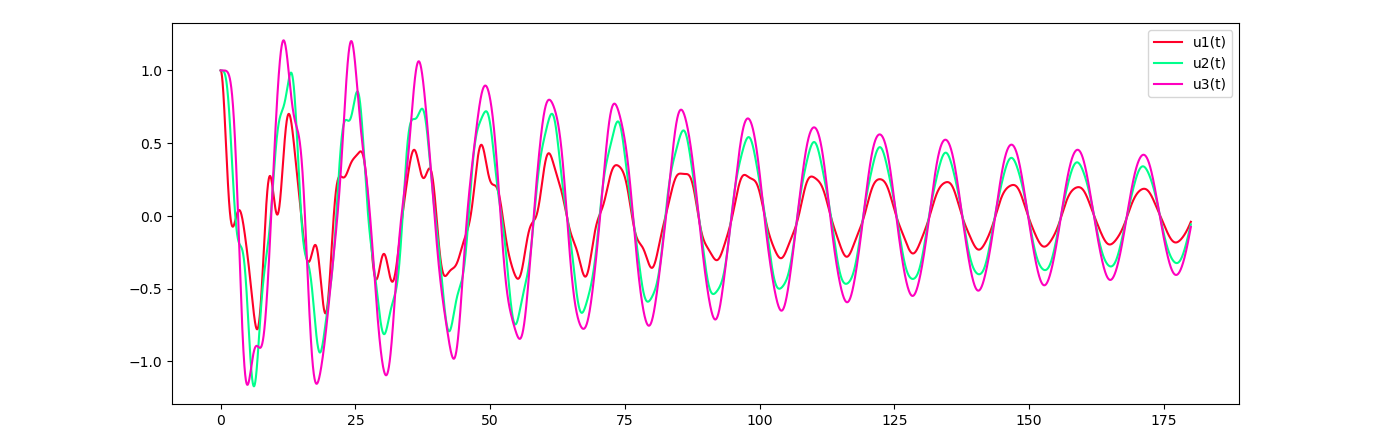
\includegraphics[width=\textwidth]{sol_sismo_natural_frequency}
    \caption{Gráfica de \(\mathbf{u}(t)\) con \(\mathbf{P}(t) = \mathbf{0}\) y condiciones iniciales \(\mathbf{u}(0) = \mathbf{1}\) para \(t \in [0, 180]\)}
    \label{fig:sol-natural-frequency}
\end{figure}

De la gráfica, contamos la cantidad de oscilaciones completas realizadas (llámese \(N\)) y el tiempo transcurrido durante estas oscilaciones (llámese \(\Delta t\)), de tal forma que se pudiese calcular la frecuencia natural \(f_n\) de la estructura con una precisión aceptable mediante
\[
    f_n = \frac{N}{\Delta t}
.\]

De la figura~\ref{fig:sol-natural-frequency}, en particular, se pueden observar \(14\) oscilaciones completas en un lapso de \(\Delta t = 171\) segundos, por lo que la frecuencia natural de la estructura mostrada, en particular, resulta
\[
    f_n = \frac{14}{171} \, \si{Hz} \approx 0.0819 \, \si{Hz}
.\]

\end{appendices}
